
\documentclass[conference]{IEEEtran}
\usepackage{amsmath}
\usepackage{listings}

% *** CITATION PACKAGES ***
%
%\usepackage{cite}
% cite.sty was written by Donald Arseneau
% V1.6 and later of IEEEtran pre-defines the format of the cite.sty package
% \cite{} output to follow that of IEEE. Loading the cite package will
% result in citation numbers being automatically sorted and properly
% "compressed/ranged". e.g., [1], [9], [2], [7], [5], [6] without using
% cite.sty will become [1], [2], [5]--[7], [9] using cite.sty. cite.sty's
% \cite will automatically add leading space, if needed. Use cite.sty's
% noadjust option (cite.sty V3.8 and later) if you want to turn this off.
% cite.sty is already installed on most LaTeX systems. Be sure and use
% version 4.0 (2003-05-27) and later if using hyperref.sty. cite.sty does
% not currently provide for hyperlinked citations.
% The latest version can be obtained at:
% http://www.ctan.org/tex-archive/macros/latex/contrib/cite/
% The documentation is contained in the cite.sty file itself.




\usepackage{graphicx}

% *** GRAPHICS RELATED PACKAGES ***
%
\ifCLASSINFOpdf
  % \usepackage[pdftex]{graphicx}
  % declare the path(s) where your graphic files are
  % \graphicspath{{../pdf/}{../jpeg/}}
  % and their extensions so you won't have to specify these with
  % every instance of \includegraphics
  % \DeclareGraphicsExtensions{.pdf,.jpeg,.png}
\else
  % or other class option (dvipsone, dvipdf, if not using dvips). graphicx
  % will default to the driver specified in the system graphics.cfg if no
  % driver is specified.
  % \usepackage[dvips]{graphicx}
  % declare the path(s) where your graphic files are
  % \graphicspath{{../eps/}}
  % and their extensions so you won't have to specify these with
  % every instance of \includegraphics
  % \DeclareGraphicsExtensions{.eps}
\fi
% graphicx was written by David Carlisle and Sebastian Rahtz. It is
% required if you want graphics, photos, etc. graphicx.sty is already
% installed on most LaTeX systems. The latest version and documentation can
% be obtained at: 
% http://www.ctan.org/tex-archive/macros/latex/required/graphics/
% Another good source of documentation is "Using Imported Graphics in
% LaTeX2e" by Keith Reckdahl which can be found as epslatex.ps or
% epslatex.pdf at: http://www.ctan.org/tex-archive/info/
%
% latex, and pdflatex in dvi mode, support graphics in encapsulated
% postscript (.eps) format. pdflatex in pdf mode supports graphics
% in .pdf, .jpeg, .png and .mps (metapost) formats. Users should ensure
% that all non-photo figures use a vector format (.eps, .pdf, .mps) and
% not a bitmapped formats (.jpeg, .png). IEEE frowns on bitmapped formats
% which can result in "jaggedy"/blurry rendering of lines and letters as
% well as large increases in file sizes.
%
% You can find documentation about the pdfTeX application at:
% http://www.tug.org/applications/pdftex





% *** MATH PACKAGES ***
%
%\usepackage[cmex10]{amsmath}
% A popular package from the American Mathematical Society that provides
% many useful and powerful commands for dealing with mathematics. If using
% it, be sure to load this package with the cmex10 option to ensure that
% only type 1 fonts will utilized at all point sizes. Without this option,
% it is possible that some math symbols, particularly those within
% footnotes, will be rendered in bitmap form which will result in a
% document that can not be IEEE Xplore compliant!
%
% Also, note that the amsmath package sets \interdisplaylinepenalty to 10000
% thus preventing page breaks from occurring within multiline equations. Use:
%\interdisplaylinepenalty=2500
% after loading amsmath to restore such page breaks as IEEEtran.cls normally
% does. amsmath.sty is already installed on most LaTeX systems. The latest
% version and documentation can be obtained at:
% http://www.ctan.org/tex-archive/macros/latex/required/amslatex/math/





% *** SPECIALIZED LIST PACKAGES ***
%
%\usepackage{algorithmic}
% algorithmic.sty was written by Peter Williams and Rogerio Brito.
% This package provides an algorithmic environment fo describing algorithms.
% You can use the algorithmic environment in-text or within a figure
% environment to provide for a floating algorithm. Do NOT use the algorithm
% floating environment provided by algorithm.sty (by the same authors) or
% algorithm2e.sty (by Christophe Fiorio) as IEEE does not use dedicated
% algorithm float types and packages that provide these will not provide
% correct IEEE style captions. The latest version and documentation of
% algorithmic.sty can be obtained at:
% http://www.ctan.org/tex-archive/macros/latex/contrib/algorithms/
% There is also a support site at:
% http://algorithms.berlios.de/index.html
% Also of interest may be the (relatively newer and more customizable)
% algorithmicx.sty package by Szasz Janos:
% http://www.ctan.org/tex-archive/macros/latex/contrib/algorithmicx/




% *** ALIGNMENT PACKAGES ***
%
%\usepackage{array}
% Frank Mittelbach's and David Carlisle's array.sty patches and improves
% the standard LaTeX2e array and tabular environments to provide better
% appearance and additional user controls. As the default LaTeX2e table
% generation code is lacking to the point of almost being broken with
% respect to the quality of the end results, all users are strongly
% advised to use an enhanced (at the very least that provided by array.sty)
% set of table tools. array.sty is already installed on most systems. The
% latest version and documentation can be obtained at:
% http://www.ctan.org/tex-archive/macros/latex/required/tools/


%\usepackage{mdwmath}
%\usepackage{mdwtab}
% Also highly recommended is Mark Wooding's extremely powerful MDW tools,
% especially mdwmath.sty and mdwtab.sty which are used to format equations
% and tables, respectively. The MDWtools set is already installed on most
% LaTeX systems. The lastest version and documentation is available at:
% http://www.ctan.org/tex-archive/macros/latex/contrib/mdwtools/


% IEEEtran contains the IEEEeqnarray family of commands that can be used to
% generate multiline equations as well as matrices, tables, etc., of high
% quality.


%\usepackage{eqparbox}
% Also of notable interest is Scott Pakin's eqparbox package for creating
% (automatically sized) equal width boxes - aka "natural width parboxes".
% Available at:
% http://www.ctan.org/tex-archive/macros/latex/contrib/eqparbox/





% *** SUBFIGURE PACKAGES ***
%\usepackage[tight,footnotesize]{subfigure}
% subfigure.sty was written by Steven Douglas Cochran. This package makes it
% easy to put subfigures in your figures. e.g., "Figure 1a and 1b". For IEEE
% work, it is a good idea to load it with the tight package option to reduce
% the amount of white space around the subfigures. subfigure.sty is already
% installed on most LaTeX systems. The latest version and documentation can
% be obtained at:
% http://www.ctan.org/tex-archive/obsolete/macros/latex/contrib/subfigure/
% subfigure.sty has been superceeded by subfig.sty.



%\usepackage[caption=false]{caption}
%\usepackage[font=footnotesize]{subfig}
% subfig.sty, also written by Steven Douglas Cochran, is the modern
% replacement for subfigure.sty. However, subfig.sty requires and
% automatically loads Axel Sommerfeldt's caption.sty which will override
% IEEEtran.cls handling of captions and this will result in nonIEEE style
% figure/table captions. To prevent this problem, be sure and preload
% caption.sty with its "caption=false" package option. This is will preserve
% IEEEtran.cls handing of captions. Version 1.3 (2005/06/28) and later 
% (recommended due to many improvements over 1.2) of subfig.sty supports
% the caption=false option directly:
%\usepackage[caption=false,font=footnotesize]{subfig}
%
% The latest version and documentation can be obtained at:
% http://www.ctan.org/tex-archive/macros/latex/contrib/subfig/
% The latest version and documentation of caption.sty can be obtained at:
% http://www.ctan.org/tex-archive/macros/latex/contrib/caption/




% *** FLOAT PACKAGES ***
%
%\usepackage{fixltx2e}
% fixltx2e, the successor to the earlier fix2col.sty, was written by
% Frank Mittelbach and David Carlisle. This package corrects a few problems
% in the LaTeX2e kernel, the most notable of which is that in current
% LaTeX2e releases, the ordering of single and double column floats is not
% guaranteed to be preserved. Thus, an unpatched LaTeX2e can allow a
% single column figure to be placed prior to an earlier double column
% figure. The latest version and documentation can be found at:
% http://www.ctan.org/tex-archive/macros/latex/base/



%\usepackage{stfloats}
% stfloats.sty was written by Sigitas Tolusis. This package gives LaTeX2e
% the ability to do double column floats at the bottom of the page as well
% as the top. (e.g., "\begin{figure*}[!b]" is not normally possible in
% LaTeX2e). It also provides a command:
%\fnbelowfloat
% to enable the placement of footnotes below bottom floats (the standard
% LaTeX2e kernel puts them above bottom floats). This is an invasive package
% which rewrites many portions of the LaTeX2e float routines. It may not work
% with other packages that modify the LaTeX2e float routines. The latest
% version and documentation can be obtained at:
% http://www.ctan.org/tex-archive/macros/latex/contrib/sttools/
% Documentation is contained in the stfloats.sty comments as well as in the
% presfull.pdf file. Do not use the stfloats baselinefloat ability as IEEE
% does not allow \baselineskip to stretch. Authors submitting work to the
% IEEE should note that IEEE rarely uses double column equations and
% that authors should try to avoid such use. Do not be tempted to use the
% cuted.sty or midfloat.sty packages (also by Sigitas Tolusis) as IEEE does
% not format its papers in such ways.





% *** PDF, URL AND HYPERLINK PACKAGES ***
%
%\usepackage{url}
% url.sty was written by Donald Arseneau. It provides better support for
% handling and breaking URLs. url.sty is already installed on most LaTeX
% systems. The latest version can be obtained at:
% http://www.ctan.org/tex-archive/macros/latex/contrib/misc/
% Read the url.sty source comments for usage information. Basically,
% \url{my_url_here}.





% *** Do not adjust lengths that control margins, column widths, etc. ***
% *** Do not use packages that alter fonts (such as pslatex).         ***
% There should be no need to do such things with IEEEtran.cls V1.6 and later.
% (Unless specifically asked to do so by the journal or conference you plan
% to submit to, of course. )


% correct bad hyphenation here
%\hyphenation{op-tical net-works semi-conduc-tor}


\begin{document}
%
% paper title
% can use linebreaks \\ within to get better formatting as desired
\title{An Empirical Study on the Usage of Mocking Frameworks in Software Testing}


% author names and affiliations
% use a multiple column layout for up to three different
% affiliations
\author{\IEEEauthorblockN{Shaikh Mostafa, Xiaoyin Wang}
\IEEEauthorblockA{Department of Computer Science, University of Texas at San Antonio, San Antonio, Texas, USA 78249\\
Email: \{Shaikh.Mostafa, Xiaoyin.Wang\}@utsa.edu}
}

% conference papers do not typically use \thanks and this command
% is locked out in conference mode. If really needed, such as for
% the acknowledgment of grants, issue a \IEEEoverridecommandlockouts
% after \documentclass

% for over three affiliations, or if they all won't fit within the width
% of the page, use this alternative format:
% 
%\author{\IEEEauthorblockN{Michael Shell\IEEEauthorrefmark{1},
%Homer Simpson\IEEEauthorrefmark{2},
%James Kirk\IEEEauthorrefmark{3}, 
%Montgomery Scott\IEEEauthorrefmark{3} and
%Eldon Tyrell\IEEEauthorrefmark{4}}
%\IEEEauthorblockA{\IEEEauthorrefmark{1}School of Electrical and Computer Engineering\\
%Georgia Institute of Technology,
%Atlanta, Georgia 30332--0250\\ Email: see http://www.michaelshell.org/contact.html}
%\IEEEauthorblockA{\IEEEauthorrefmark{2}Twentieth Century Fox, Springfield, USA\\
%Email: homer@thesimpsons.com}
%\IEEEauthorblockA{\IEEEauthorrefmark{3}Starfleet Academy, San Francisco, California 96678-2391\\
%Telephone: (800) 555--1212, Fax: (888) 555--1212}
%\IEEEauthorblockA{\IEEEauthorrefmark{4}Tyrell Inc., 123 Replicant Street, Los Angeles, California 90210--4321}}




% use for special paper notices
%\IEEEspecialpapernotice{(Invited Paper)}




% make the title area
\maketitle


\begin{abstract}
In software testing, especially unit testing, it is very common that software testers need to test a class or a component without integration with some of its dependencies. Typical reasons for excluding dependencies in testing include the unavailability of some dependency due to concurrent software development and callbacks in frameworks, high cost of invoking some dependencies (e.g., slow network or database operations, commercial third-party web services), and the potential interference of bugs in the dependencies.  In practice, mock objects have been used in software testing to simulate such missing dependencies, and a number of popular mocking frameworks (e.g., Mockito, EasyMock) have been developed for software testers to generate mock objects more conveniently. However, despite the wide usage of mocking frameworks in software practice, there have been very few academic studies to observe and understand the usage status of mocking frameworks, and the major issues software testers are facing when using such mocking frameworks. In this paper, we report on an empirical study on the usage of four most popular mock frameworks (Mockito, EasyMock, JMock, and JMockit) in 5,000 open source software projects from GitHub. The results of our study show that the above mentioned mocking frameworks are used in a large portion (about 23\%) of software projects that have test code. We also find that software testers typically create mocks for only part of the software dependencies, and there are more mocking of source code classes than library classes. 

\end{abstract}

% IEEEtran.cls defaults to using nonbold math in the Abstract.
% This preserves the distinction between vectors and scalars. However,
% if the conference you are submitting to favors bold math in the abstract,
% then you can use LaTeX's standard command \boldmath at the very start
% of the abstract to achieve this. Many IEEE journals/conferences frown on
% math in the abstract anyway.

% no keywords




% For peer review papers, you can put extra information on the cover
% page as needed:
% \ifCLASSOPTIONpeerreview
% \begin{center} \bfseries EDICS Category: 3-BBND \end{center}
% \fi
%
% For peerreview papers, this IEEEtran command inserts a page break and
% creates the second title. It will be ignored for other modes.
%\IEEEpeerreviewmaketitle






% An example of a floating figure using the graphicx package.
% Note that \label must occur AFTER (or within) \caption.
% For figures, \caption should occur after the \includegraphics.
% Note that IEEEtran v1.7 and later has special internal code that
% is designed to preserve the operation of \label within \caption
% even when the captionsoff option is in effect. However, because
% of issues like this, it may be the safest practice to put all your
% \label just after \caption rather than within \caption{}.
%
% Reminder: the "draftcls" or "draftclsnofoot", not "draft", class
% option should be used if it is desired that the figures are to be
% displayed while in draft mode.
%
%\begin{figure}[!t]
%\centering
%\includegraphics[width=2.5in]{myfigure}
% where an .eps filename suffix will be assumed under latex, 
% and a .pdf suffix will be assumed for pdflatex; or what has been declared
% via \DeclareGraphicsExtensions.
%\caption{Simulation Results}
%\label{fig_sim}
%\end{figure}

% Note that IEEE typically puts floats only at the top, even when this
% results in a large percentage of a column being occupied by floats.


% An example of a double column floating figure using two subfigures.
% (The subfig.sty package must be loaded for this to work.)
% The subfigure \label commands are set within each subfloat command, the
% \label for the overall figure must come after \caption.
% \hfil must be used as a separator to get equal spacing.
% The subfigure.sty package works much the same way, except \subfigure is
% used instead of \subfloat.
%
%\begin{figure*}[!t]
%\centerline{\subfloat[Case I]\includegraphics[width=2.5in]{subfigcase1}%
%\label{fig_first_case}}
%\hfil
%\subfloat[Case II]{\includegraphics[width=2.5in]{subfigcase2}%
%\label{fig_second_case}}}
%\caption{Simulation results}
%\label{fig_sim}
%\end{figure*}
%
% Note that often IEEE papers with subfigures do not employ subfigure
% captions (using the optional argument to \subfloat), but instead will
% reference/describe all of them (a), (b), etc., within the main caption.


% An example of a floating table. Note that, for IEEE style tables, the 
% \caption command should come BEFORE the table. Table text will default to
% \footnotesize as IEEE normally uses this smaller font for tables.
% The \label must come after \caption as always.
%
%\begin{table}[!t]
%% increase table row spacing, adjust to taste
%\renewcommand{\arraystretch}{1.3}
% if using array.sty, it might be a good idea to tweak the value of
% \extrarowheight as needed to properly center the text within the cells
%\caption{An Example of a Table}
%\label{table_example}
%\centering
%% Some packages, such as MDW tools, offer better commands for making tables
%% than the plain LaTeX2e tabular which is used here.
%\begin{tabular}{|c||c|}
%\hline
%One & Two\\
%\hline
%Three & Four\\
%\hline
%\end{tabular}
%\end{table}


% Note that IEEE does not put floats in the very first column - or typically
% anywhere on the first page for that matter. Also, in-text middle ("here")
% positioning is not used. Most IEEE journals/conferences use top floats
% exclusively. Note that, LaTeX2e, unlike IEEE journals/conferences, places
% footnotes above bottom floats. This can be corrected via the \fnbelowfloat
% command of the stfloats package.

\vspace{-0.3cm}

\section{Introduction}
\label{sec:intro}
During software evolution, frequent code changes, often including problematic changes, may degrade software performance. For example, a study~\cite{huang2014performance} found that upgrading from MySQL 4.1 to 5.0 caused the loading time of the same web page to increase from 1 second to 20 seconds in a production e-commerce website. Even small performance degradation may result in severe consequence. For example, Google could lose 20\% traffic due to an increase of 500ms latency~\cite{Google}. Amazon could have 1\% decrease in sales due to a 100ms delay in page rendering~\cite{Stevefamov}. \\

Developers can apply systematic, continuous performance regression testing to reveal such performance regressions in early stages~\cite{foxref,poliniref,TSEPerform,MITCHELL,KALIBERA}. But due to its high overhead, performance regression testing is expensive to conduct frequently. Actually, the typical execution cost of popular performance benchmarks varies from tens of minutes to tens of hours~\cite{huang2014performance}, so it is impractical to run all performance test cases for each code commit. Recently, PerfScope~\cite{huang2014performance} was proposed to predict whether a code commit may significantly affect software performance and thus require performance testing. Specifically, PerfScope extracts various features from the original version and the code commit, and trains a classification model for prediction. Although PerfScope helps reduce code commits for performance regression testing, its empirical evaluation shows that a non-trivial proportion of code commits still require performance testing; thus, there is still a strong need of reducing the cost of conducting performance regression testing on a code commit, even after applying PerfScope in practice.\\

%Such problematic changes are referred to as performance regressions in this paper. and GCC from 4.3 to 4.5, Mozilla developers experienced an up to 19\% performance regression, which forced them to consider a complete switchover.Performance regression testing is a major approach to detecting performance regressions, This is widely advocated in academia, open source community and industry .for web servers is 3 minute to 1 hr, for databases is 10 minutes to 3 hrs, for compilers is 1 hr to 20 hrs and for operating systems is 2 hrs to 24 hrs . With the high revision frequency and high testing cost, 


%
%it does not consider the performance impact of code commits on individual test cases, and thus results in two limitations. First,
%

To address such strong need, developers shall prioritize performance test cases on a code commit for three main reasons. First, there can be high cost to execute all performance test cases on a code commit for large systems in practice. Second, as reported in a previous industrial study~\cite{TSEPerform} and our study in Section~\ref{sec:motivation}, various random factors may affect the observed execution time, so it typically requires a large number of repetitive executions to confirm a performance regression. Therefore, with prioritized test cases, developers can better distribute testing resources  (i.e., do more executions on test cases likely to trigger performance regressions). 
Third, a code commit may accelerate some test cases while slowing down others. It is often important for the developers to understand the performance of their software under different scenarios, while a coarse-grained commit-level technique is not helpful on this requirement. \\



%research effort by addressed this problem with PerfScope, or regressional performance testing. Specifically, for each new code commit, PerfScope applied to the code change various program analysis (e.g., hot path analysis, bound analysis, and data dependency analysis) to  to 

%For example, our study shows that it averagely requires 150 executions to confirm a 10\% performance difference, which is typically considered significant, and dynamic techniques bringing in more than 10\% overhead are typically not considered for deployment-time usage~\cite{}. 


%Mozilla’s Talos performance regression detection system~\cite{firefoxTalos} runs performance tests every time a change is pushed to the Firefox source repository~\cite{firefoxperf}. In our empirical evaluation, we observe that one code commit may affect more than 100 test cases. 


 


%There is a useful work on the performance risk implication of code change. But their approach may not accurately assess the risk of performance regression issues because of generic nature of static modeling and lacking profiling information. Furthermore, prioritizing commits is not enough to address performance regression because  a code changes touches several test cases is very common during the evolution of software. In our study, we found that some commits touches more than 100 test cases. So the key difference is that we focus  on the prioritizing test cases in regressional performance testing via performance impact analysis of code changes that includes one time profiling and static modeling.

To develop an effective test-prioritization solution for performance regression testing, we focus on \textit{collection-intensive software}, an important type of modern software whose execution time is heavily spent on loading, manipulating, and writing collections of data. Collections are widely used in software for scalable data storage and processing, and thus collection-intensive software is very common. Examples include libraries for data structures, text formating and parsing, mathematics, image processing, etc. Also, collection-intensive software is often used as components in complex systems. Moreover, a recent study~\cite{JIN12} shows that a large portion of performance bugs are related to loops, which are often used to iterate through collections. Our statistics show that 89\% and 77\% of loops iterate through collections for our two subjects Xalan and Apache Commons Math, respectively.\\

%improper iteration on collections has been identified as one of the most
%

For collection-intensive software, a straightforward approach to prioritizing performance test cases on a code commit would be measuring collection iterations (e.g., loops) impacted by the code commit and executed by each test case. However, such an approach may not be precise enough to differentiate test cases in the presence of newly added iterations, manipulations, and processing of collections, as well as their effect on existing collection iterations. Consider the simplified code example from Xalan in Listing~\ref{list:example-p3}. The code commit involves a new loop, and its location may or may not be at the hot spot for all or most test cases. Therefore, its impact on different test cases may largely depend on the different iteration counts of the added loop, the side effect of changing variable \CodeIn{list}, and the operations in the loop. Since Loop$_B$ depends on a collection variable \CodeIn{limits}, which further depends on Loop$_A$, we can infer the test-case-specific iteration count of Loop$_B$ from that of Loop$_A$; such iteration count can be acquired by profiling the base version for all test cases. Furthermore, we can infer the effect of adding \CodeIn{list.add(...)} on \CodeIn{list} with the iteration count of Loop$_B$, and update the iteration count of loops dependent on \CodeIn{list}. Moreover, we can enhance the estimation precision by using test-case-specific execution time of operations (e.g., \CodeIn{new Arc(...)}). 


{\fontsize{10}{10}
	\begin{lstlisting}[columns=flexible,language=Java,caption=Collection Loop Correlation, label={list:example-p3}]
	  while(i <= m\_size){ //Loop A
	    limits.add(new Limit(...))
	    ...
	  }
	  ...
	+ Collections.sort(limits);
	+ for (int i = 0; i < limits.size()-1; i++) { //Loop B
	+   list.add(new Arc(limits.get(i), ...));
	+ }
	\end{lstlisting}
}


These observations inspire us for three main insights to effectively model a code commit and its effect on existing collections and their iterations. First, collection sizes (e.g., \CodeIn{limits.size()}) and loop-iteration counts (e.g., Loop$_B$) can often be correlated, so collection sizes can be inferred from loop-iteration numbers and vice versa. Also, collection variables (e.g., \CodeIn{limits}) can be used as bridges to infer iteration counts of new loops (e.g., Loop$_B$) from existing loops (e.g., Loop$_A$). Second, collection manipulations (e.g., \CodeIn{list.add(...)}) are often inside loops, so the size of collections referred by collection variables (e.g. \CodeIn{list}) can be estimated from loop-iteration counts (e.g., Loop$_B$). Third, due to the large number of elements in collections, the average processing time of elements (e.g., \CodeIn{new Arc(...)}) is relatively stable, so a method's average execution time in the new version may be estimated from that in the base version.\\ 

Based on the three insights, we propose PerfRanker, which consists of four automatic steps. First, on a base version, we execute each test case in a profiling mode to collect information about the test execution, including the runtime call graph and the iteration counts of all executed loops. We also perform static analysis to capture the dependency among collection objects and loops. Second, based on the profiling information, we construct a performance model for each test case. Third, given a code commit, we estimate the execution time of each test case on the new version (formed by the code commit) by extending and revising its old performance model. We use profiling information and loop-collection correlations to infer parameters of the new performance model, and refer to this step as \textit{Performance Impact Analysis}. Fourth, we rank all the test cases based on the performance impact on them.\\

%its impact on each test case from two aspects: the execution time of the added and removed code in the revised method, and the execution time of the loops affected by the collection objects which are return values of revised methods. 




%To address the two limitations above, we propose a novel approach to prioritize individual test cases in performance regression testing via performance impact analysis, which estimates the impact of a given code revision on the execution time of a given test case. 



%our algorithm automatically takes the information in each code commit by statically analyzing the added code and removed code from automatically generated diff of each commit. Incorporating the profile and static information into each test case's call graph we determine the run-time cost and the execution frequency of the code affected by code changes. 

We implement our approach and apply it on two sets of code commits collected from popular open source collection-intensive projects: Apache Commons Math and Xalan. To measure the effectiveness of test case prioritization for a code commit in performance regression testing, we use three metrics: (1) \textit{APFD-P} (Average Percentage Fault Detected for Performance), an adapted version of the APFD metric~\cite{AlexeyAPFD} for performance testing, (2) \textit{DCG}~\cite{NDCG}, a general metric for comparing the similarity of two sequences, and (3) \textit{Top-N Percentile}, which calculates the percentage of test cases needed to be executed to cover the top N test cases whose execution time is most affected by the code commit. Our evaluation results show that, compared with the best of the three other baseline approaches, our approach achieves an average improvement of 17.6 percentage points on \textit{APFD-P} and 27.4 percentage points on DCG. Furthermore, for Apache Commons Math and Xalan, our approach is able to rank top 1 affected test case within top 8\% and top 16\% test cases, and top 3 affected test cases within top 37\% and 30\% test cases, respectively. 

%Since we are not aware of previous research efforts on prioritizing test cases for performance regression testing, we developed  for Apache Commons Math, and an improvement of 16.6 percentage points on APFD and 27.2 percentage points on DCG for Xalan, respectively

%calculated impact score is used with adaptive APFD and DCG metric formula to rank the test case which shows that they can significantly reduce the cost of performance regression. 


This paper makes the following major contributions:
  \vspace{-0.1cm}
\begin{itemize}
  \item A novel approach to prioritizing test cases in performance regression testing of collection-intensive software.
  
  
%supported by a novel technique called performance impact analysis which estimates the performance impact of code revisions on test cases.
  
%  \item A motivation study on the number of executions required to acquire stable performance testing results.
    
    
  \item Adaptation of the APFD metric to measure the result of test prioritization for performance regression testing. 
    
  \item An evaluation of our approach on real-world code commits from two popular open source collection-intensive projects. 
  
\end{itemize}
  
  
%The rest parts of this paper are organized as follows. In Section~\ref{sec:motivation}, we present a motivation study showing that multiple test executions are required to confirm a performance regression. In Section~\ref{sec:approach}, we introduce our approach and performance impact analysis in details. We present our evaluation results in Section~\ref{sec:evaluation}, and discuss some related issues in Section~\ref{sec:discuss}. Before we conclude in Section~\ref{sec:conclusion}, we introduce related research efforts in Section~\ref{sec:related}, and indicate some future work in Section~\ref{sec:future}.
\vspace{-0.3cm}

\section{Background}
\label{sec:backgroundmock}
In this section, we first introduce some basic background knowledge on mocking objects. Then, we introduce the mechanism of mocking frameworks and some major mocking frameworks.
\subsection{Mocking Objects}

Mocking objects are used in software testing to simulate software dependencies so that the testing process can be accelerated and the testing scope can be limited to the component under test (instead of going beyond the interface of dependencies and invoke potential bugs relevant to dependencies). To simulate real dependencies, mock objects typically have the same interface as the objects they mimic. Therefore, the client object remains unaware of whether it is using a real object or a mock object. 

%The major difference between mock object and other test doubles (i.e., objects simulating software dependencies, such as test stubs, fake objects) is that, on top of simulating software dependencies, mock objects also contain assertions of their own. Mock objects will examine the context of each invocation of their methods, on whether a method is invoked, whether several methods are invoked in correct order, and whether arguments of the methods are passed in correctly. 

For example, when testing an email client, software testers may not use the real email server which has slow response and random failures. By contrast, they may construct a fake email server object (a mock object) that returns whatever expected by the software testers. The expected return value can be either a simple success code for the testing of normal functioning of the email client, or a server error code for the testing of error handling of the email client. Such a fake email server helps to reduce testing time as well as to explore the handling of server errors that are very hard to invoke with a real server. However, when such a simplified email server is used, it is hard for testers to tell whether the email client has invoked the email server in a correct order (if multiple-step configuration of the server is required), or whether the client has passed correct arguments to the server. 

Therefore, the software testers may further have some code in the fake email server to check whether the client interacts with it correctly and passes correct arguments. With such a mock email server, software testers can perform quick and controllable testing of the email client without losing the thorough exploration of the interface between the email client and the email server.


\subsection{Mocking Frameworks}

As mentioned in the previous section, mocking objects are desirable for simulating software dependencies in software testing. However, since mock objects need to perform various checking of the invocations, it is usually nontrivial to write such mock objects, and thus the benefit of using mock objects can be undermined by the effort spent on writing mock objects. 

To solve this problem, in the past decade, people have developed various mocking frameworks to generate mock objects automatically. A code sample of using a mocking framework is presented below. With a mocking framework, software testers first create an empty mock object (Line 3). Then, for the created mock object, software testers can specify a number of invocation for the object to check, both on the order of the invocations and the correctness of the arguments (Line 6). After that, in the test code, testers run the component under test as usual but with created mock objects (Line 8). During the execution, if the specified invocation order or arguments are not satisfied, the mock object will throw a test failure so that the software testers know that something wrong happened (Line 9). \\


\begin{lstlisting}[language=Java]
1: @Test
2: public void testEmailClient(){
3:     Server sv = EasyMock.
            CreateMock(Server.class); 
4:     Client c = new Client(sv);         
5:     Email em = new Email(...)
        //record
6:     EasyMock.expect(sv.send(em)).
            andReturn(0);
        //replay
7:     EasyMock.replay(sv);
8:     c.send(em)
9:     EasyMock.verify(sv)
10:}
\end{lstlisting}


For each major programming language, there have been a number of mocking frameworks developed, such as Mockito, EasyMock, and JMock for Java, pmock, mox for Python, and NMock, Moq for C\#. All of these mocking frameworks support the basic features of mocking including the creation of mock objects, the specification of invocation orders and arguments, and the verification of the specifications. The differences between these mocking frameworks are mainly on the design of APIs and supporting of advanced specifications such as checking the number of invocations of a certain method. 

\vspace{-0.3cm}

\section{Design}
\label{sec:design}
In this section, we introduce the design of our empirical study on the usage of mocking frameworks among developers of open source software projects. 
\vspace{-0.2cm}

\subsection{Research Questions}
\label{subsec:rq}
\vspace{-0.2cm}

In this study, we design an experiment to answer the following research questions. By answering these questions, we try to understand whether and how software developers and testers use mocking frameworks to handle dependencies in the testing of open source software projects. 
\begin{itemize}
\item \textbf{RQ1:} How popular are mocking frameworks that are used in the testing of open source Java software projects? Are developers trying to mock most or all of dependencies?
\item \textbf{RQ2:} What features of mocking frameworks are most frequently used in the testing of open source software projects?
\item \textbf{RQ3:} What types of dependencies developers tend to mock?
\end{itemize}
\vspace{-0.2cm}

\subsection{Subjects}
\vspace{-0.2cm}

To perform our empirical study, we randomly downloaded 5,000 Java software projects from Github. We choose to focus on Java software projects because Java is one of the most widely used object-oriented programming language, and due to the popularity of Java in the open source community, a large number of open source Java software projects may serve as subjects. When selecting subject projects, we first search Java projects in Github with 26 keywords from 'a' to 'z', and then, we randomly sample 5000 projects from the merged search results. For each project, we consider only the most recent version. 

The basic information of the 5,000 Java software projects are presented in Table~\ref{table:basic}.

\begin{table}
\caption{Basic Information of Subjects Used in Study}
\label{table:basic}
\centering
\begin{tabular}{|c|r|r|r|r|}
\hline
Info Type & Avg. & Med. & Max. & Min\\
\hline
\# Java Files &153&18&10,141&1\\
LOC  &25,305&1,833&3,094,265&0\\
\# Test Files  &16.4&0&3,335&0\\
\# Developers  &3.0&1&39&1\\
\# Versions  &11.4&1&1694&1\\
\hline
\end{tabular}
\end{table}

In Table~\ref{table:basic}, we present five types of basic information of the collected software projects, which are in the Lines 2-6 of the table. Specifically, Line 2 presents the number of Java Files in the project. It should be noted that some of the software projects may be developed in multiple programming languages and may involve other types of source code files. In our study, we focus only on the Java part of such software projects. Line 3 presents the total lines of source code in the Java source files. Line 4 presents the number of test files in the software projects. Specifically, we consider a Java source file as a test file if it uses any library classes from JUnit or TestNG, which are the two major test frameworks for Java and the only test frameworks we notice the collected software projects are using. It should be noted that, in some software projects, a test class $C$ may extend a library class in test frameworks, and other test files use only $C$ but not any library classes in test frameworks. So in our study, we also consider the test files that indirectly use library classes in test frameworks by using classes like $C$. Line 5 and Line 6 present the number of developers and the number of versions (i.e. code commits) of the software projects. 

Due to the large number of subjects, we are not able to present the basic information of individual software projects. Instead, we present the statistical information of the software projects. Column 2-5 present the average, medium, maximum and minimum of all types of information, respectively.  

From Table~\ref{table:basic}, we can see that the chosen subjects vary largely in their sizes, testing efforts, number of developers, and history. The average size of the subjects are 25KLOC, and the largest subject has more than 3 million lines of code. Furthermore, more than half of the subjects have no test code (the medium of number of test files is 0), and the average number of test classes is 16.4. 
\vspace{-0.2cm}

\subsection{Process}
\vspace{-0.2cm}

To answer the research questions listed in Section~\ref{subsec:rq}, for each of the collected subject, we first identify all the Java source files and test files. Then, we parse these files to extract the code relevant to mocking frameworks. 

In particular, we consider the four most popular Java mocking frameworks in our study: Mockito, EasyMock, JMock, and JMockit. PowerMock is another popular mocking framework, but it is actually an extension of Mockito and EasyMock frameworks, and typically software projects using PowerMock will use at least one of Mockito or EasyMock frameworks, so we do not consider PowerMock in our study. 

The four investigated frameworks have some specific characteristics. EasyMock
requires developers to specify the type of the mock object at the creation point (i.e., whether the mock object is strict or not, and whether to raise exceptions when there are unexpected methods invoked). Typically, EasyMock is more strict to raise more run time errors, and the interface is not very easy to learn (comments from StackOverflow). Mockito actually origins from EasyMock, and it
provides a very simple API interface to create mocking objects (not strict by default) and support annotations to specify the classes to be mocked. Mockito also provides very good spy features that verifies the dependency-related interaction of the class under testing on the real dependency classes. JMock is similar to EasyMock in most aspects. JMockit uses class-map as its underlying technique for mocking and thus can mock final classes. 


From the relevant code, we extract the information that can help answer our research questions, Specifically, we extract a data set of API signatures of each mocking framework from their API documents, and developed a AST-tree-based code analyzer analyze the source code of subject projects extract all relevant API invocations. Based on these API invocations, we are able to identify the API method in mocking frameworks used, the dependency classes being mocked, etc. 
\vspace{-0.3cm}

\section{Empirical Study Results}
\label{sec:studymock}


In this section, we present the details and results of our empirical study. Specifically, we present the study to answer the research questions 1 to 3 in Section~\ref{subsec:pop}, Section~\ref{subsec:usage}, and Section~\ref{subsec:mock}, respectively. We summarize our findings in Section~\ref{subsec:summary}, and present the threats to validity in Section~\ref{subsec:threat}. 

\subsection{Popularity of Mocking Frameworks}
\label{subsec:pop}


To answer the first research question, we study the number of software projects using mocking frameworks among the 5,000 downloaded software projects. Specifically, among the 5,000 software projects, 2,046 has at least one test class (a class importing and use any class from JUnit or TestNg). Among the 2,046 projects, 459 projects (23\%) uses at least one mocking framework. We guess that developers of large software projects tend to use mocking frameworks, so we compare the size distribution of software projects using mocking frameworks with the size distribution of all software projects having test code, and present the results in Figure~\ref{fig:box}. The figure shows that the size of software projects using mocking frameworks tends to be larger than other software projects with test code. Specifically, the median size of software projects using mocking frameworks is 16KLOC,  compared to 8.4KLOC of all software projects with test code (software projects in the latter set include software projects in the former set). At the same time, we also found that there are many large software projects do not use any of the investigated mocking frameworks. Furthermore, among the software projects (with test code) that are larger than 10KLOC, and 100KLOC, the proportion of software projects using mocking frameworks goes up to 30\% and 34\%, respectively. 

\begin{figure}


  \center
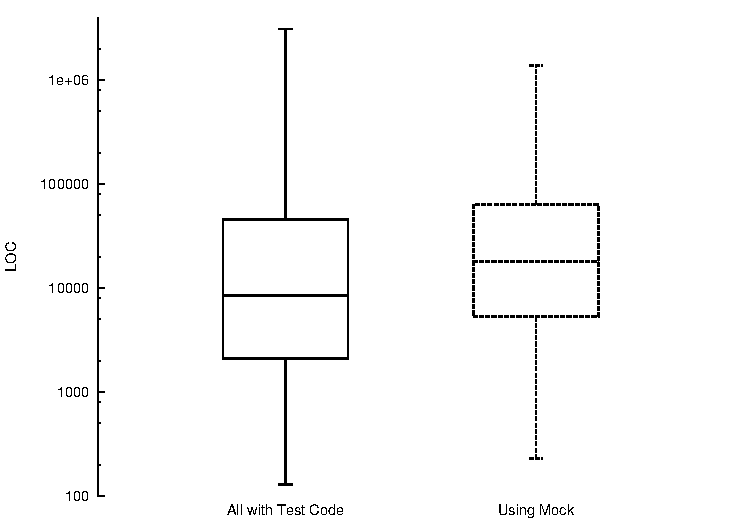
\includegraphics[width=100mm, height=60mm]{mocking/boxplot.pdf}

  \caption{\label{fig:box} Size comparison of software projects using mocking frameworks and all software projects with test code}


\end{figure}

                       
On top of the popularity of mocking frameworks in open source software projects, we are also interested in the market share of various popular mocking frameworks. Therefore, we studied the usage of different mocking frameworks and presented the results in Table~\ref{table:var}. From the table, we can see that, among the four major mocking frameworks, Mockito is the most widely used and is used in more than 70\% of software projects that use mocking frameworks. EasyMock and JMock rank second and third, and are used in about 20\% and 10\% of software projects using frameworks, respectively. JMockit is the least widely used among the four. It should be noted that this observation may not be generalized because it is from 5,000 randomly selected Java projects from GitHub. 

Furthermore, we found that 45 software projects use more than one mocking frameworks. We further studied the projects and found that the main reason for software developers to use multiple mocking frameworks is that, different software testers are more familiar with different mocking frameworks so that they use different mocking frameworks in the testing. Another reason is that the software project is moving from one framework to another. 

\begin{table}
\caption{Popularity of Mocking Frameworks}
\small

\label{table:var}
\centering
\begin{tabular}{|c|r|}
\hline
 Mocking Framework & \# Projects\\
\hline
 Using Mockito & 340\\
 Using EasyMock & 106\\
 Using JMock & 45\\
 Using JMockit & 7\\
 Total & 459\\
 Multiple Mocking Frameworks & 45\\
\hline
\end{tabular}


\end{table}

We observed that mocking frameworks are used widely in software projects. However, the data above just reveals whether a software project involves mocking frameworks in any test class. It is still not known whether mocking frameworks are used in many test classes or only  a small number of test classes. To answer this question, we further studied the number and proportion of test classes that use mocking frameworks and present the results in Table~\ref{table:testclass}

From the table, we can see that, in software projects that use mocking frameworks, on average, 16.8 test classes are using mocking frameworks, accounting for about 29.8\% of all test classes. This observation shows that software testers are not using mock objects for all dependencies. Also, it is not the case that mock objects are used very rare and in only some special cases. 

\begin{table}
\caption{Usage of Mocking Frameworks in Test Classes}
\small

\label{table:testclass}
\centering
\begin{tabular}{|c|r|r|r|r|}
\hline
 & Avg. & Med. & Max. & Min\\
\hline
\# Test Files &16.8&5&1037&1\\
Proportion of Test files &29.8\%&20\%&100\%&0.3\%\\
\hline
\end{tabular}

\end{table}

Moreover, we studied the number of mock objects in one test class and present the results in Table~\ref{table:num}. From the table, we can see that most test classes (77.2\%) have created 3 or less mock objects. Second, we try to understand, for test class that uses mocking frameworks, how many dependency classes are mocked and checked. Specifically, we deem a test class as dependency class if it is imported by the test class. The results are presented in Table~\ref{table:prop}. The table shows that on average about 17\% of dependency classes are mocked by the software testers. Thus, software testers seem to mock only a small portion of all dependency classes of a test class. 

\begin{table}

\caption{Number of Mock Objects in Test Classes}
\small

\label{table:num}
\centering
\begin{tabular}{|c|r|r|}
\hline
\# Mock Objects & \# Test Files & Proportion\\
\hline
1&1270 & 45.3\%\\
2&587 & 21.0\%\\
3&333 & 11.9\%\\
4&210 & 7.5\%\\
5&135 & 4.8\%\\
6&73 & 2.6\%\\
7&49 & 1.7\%\\
8&40 & 1.4\%\\
9&22 & 0.8\%\\
10+&82 & 2.9\%\\
\hline
\end{tabular}

\end{table}


\begin{table}
\caption{Proportion of Mocked Classes}
\small
\label{table:prop}
\centering
\begin{tabular}{|c|r|r|r|r|}
\hline
&Avg. & Med. & Max & Min\\
\hline
\# Mocked Classes &2.7&2&40&1\\
\# Dependency Classes &17.0&14&215&1\\
Proportion of Mocked Clases &17.8\%&14.3\%&100\%&0.9\%\\
\hline
\end{tabular}

\end{table}


\subsection{Usage of Mocking Frameworks}
\label{subsec:usage}


\begin{table}
\caption{Most popular ten APIs in Mockito}
\small
\label{table:mockito}
\centering
\begin{tabular}{|r|r|p{2.6in}|}
\hline
API & Frequency & Description\\
\hline
Mockito.verify&2249 & verify tester's specification of the mock object\\
Mockito.mock&1678 & create an empty mock object\\
Mockito.when&1471 & specify a method in the mock object to be invoked\\
Mockito.spy&403      & partially mock an existing class\\
Mockito.times&232   & specify how many times a method is invoked\\
Mockito.given&161   & Alias of ``when'' for behavior driven development style\\
Mockito.never&152  & specify that a method is never invoked\\
Mockito.verifyNoMoreInteractions & 98 & specify that there are no more interactions between the component under testing and the mock object\\ 
Mockito.doReturn & 85 & specify the return value of a method invocation\\
Mockito.verifyZeroInteractions & 74 & specify that there are no interactions between the component under testing and the mock object\\ 
\hline
\end{tabular}

\end{table}



To answer the second research question, we try to study what APIs in mocking frameworks are most widely used. Since different mocking frameworks have different API sets, in this phase, we study only Mockito and EasyMock, which are the most and second most widely used mocking frameworks. The results are presented in Table~\ref{table:mockito} and Table~\ref{table:easymock}


From Table~\ref{table:mockito} and Table~\ref{table:easymock}, we have the following two main observations. First of all, verification of mock objects are extensively used. This fact shows that software testers do not use mocking frameworks simply as a convenient tool for generating normal test stubs or fake objects, but are using the core features of mock objects (i.e., specifying and verifying interactions between the component under test and the software dependency). Second, several advanced APIs in Mockito are widely used. Such APIs include ``spy'' which partially mock an existing class (i.e., use the mock object for specified method invocations, but the real dependency for other method invocations), ``times'' that specify how many times a certain method is invoked, etc. 

\begin{table}
\caption{Most popular ten APIs in EasyMock}
\small
\label{table:easymock}
\centering
\begin{tabular}{|r|r|p{3in}|}
\hline
API & frequency & description\\
\hline
EasyMock.expect&671& specify a method in the mock object to be invoked\\
EasyMock.createmock&647 & create an empty mock object\\
EasyMock.replay&638 & notice the mock object that the testing of component under testing starts\\
EasyMock.verify&510&verify tester's specification of the mock object\\
EasyMock.expectLastCall&144 &alias for ``expect'' for void methods\\
EasyMock.eq & 90 & expect an value that is equals with a given value\\
EasyMock.createNiceMock & 67 &create a mock object that check the order of method invocations\\
EasyMock.anyObject & 64 & match with any type of arguments when specifying the invocation of a method\\
EasyMock.reportMatcher & 58 & specify a matcher of arguments for specification of method invocations\\
EasyMock.capture & 53 & capture a matched value for later access\\
\hline
\end{tabular}

\end{table}

\subsection{Mocked Dependencies}
\label{subsec:mock}


To answer the third research question, we studied the classes that are mocked by software testers using mocking frameworks. Specifically, we try to find out whether software testers tend to mock library classes and what are the mostly mocked library classes. To find the answer, we check whether the mocked classes are library classes (i.e., classes that are not in the source code base of the software project), and present the results in Table~\ref{table:lib}.The results show that about 39\% of all mocked classes are library classes, so software testers actually tend to mock more classes in the source code, compared with library classes. This shows that the major reason for software testers to perform mocking may be parallel development, instead of accelerating testing process and verifying interactions of classes with dependencies. 


\begin{table}
\caption{Mocking of Library Classes}
\small
\label{table:lib}
\centering
\begin{tabular}{|c|r|r|r|r|}
\hline
&Avg. & Med. & Max & Min\\
\hline
\# Mocked Library Classes &0.85&0.0&18&0\\
Proportion of Library Classes &39.4\%&0\%&100\%&0\%\\
\hline
\end{tabular}

\end{table}

In Table~\ref{table:mostlib}, we present the top 10 mostly mocked library classes. Specifically, the frequencies are the times that the specific class is mocked in all the studied open source software projects. From the table, we can observe that the two major source of mostly mocked classes are the package ``javax.servlet'', and the package ``javax.jcr''. Specifically, the former package is about HTTP request and responses, and the latter package is about the operation of Java Content Repositories. 

\begin{table}
\caption{Mostly Mocked Library Classes}
\small
\label{table:mostlib}
\centering
\begin{tabular}{|r|r|}
\hline
Mocked Library Class& Frequency \\
\hline
javax.servlet.http.HttpServletRequest&44\\
org.fest.assertions.description.Description&41\\
javax.servlet.ServletContext&33\\
javax.jcr.Node&32\\
rx.Observer&24\\
org.openqa.selenium.WebDriver&23\\
javax.servlet.http.HttpServletResponse&22\\
javax.jcr.Property&20\\
javax.jcr.Session&20\\
java.io.InputStream&17\\
\hline
\end{tabular}

\end{table}


\subsection{Summary}
\label{subsec:summary}


To sum up, the major findings of our empirical study are as below.
\begin{itemize}
\item Mocking frameworks and mock objects are used widely among open source Java software projects. However, software testers usually mock only a small number and portion of software dependencies.

\item Verification is widely used to check the specified interaction between the component under testing and the mocked object. Special APIs in both Mockito and EasyMock are widely used, which implies an incompleteness of features for a single mocking framework. 

\item Software testers tend to mock source code classes than libraries, while library classes also take a substantial proportion (40\%) in all mocked classes. The mostly mocked library classes are classes from packages handling HTTP requests / responses, and content repositories. 

\end{itemize}


\subsection{Threats to Validity}
\label{subsec:threat}


The major threat to the internal validity of our study is the potential errors in the programs analyzing the collected software projects and performing statistics. To reduce the threat, we tried our best to write the code carefully to avoid any bugs in the programs. The major threat to the external validity of our study is that our observations may be specific to the subject software projects, and cannot be generalized other software projects. To reduce this threat, we use a large number of subject software projects, and choose the subjects randomly. Also, it is possible that our findings are specific to Java software projects. To further reduce this threat, we plan to carry out similar empirical studies on subjects written with other major programming languages in the future. 



\vspace{-0.3cm}


	\vspace{-0.2cm}
\section{Related Work}
\label{sec:related}
	\vspace{-0.1cm}
	
\textbf{Performance Testing and Faults.} Previous work focuses on generating performance test infrastructures and test cases, such as automated performance benchmarking~\cite{KALIBERA}, model-based performance testing framework for workloads~\cite{BARNA11}, using genetic algorithms to expose performance regressions~\cite{LUO16}, learning-based performance testing~\cite{GRECHANIK12}, symbolic-execution-based load-test generation~\cite{ZHANG11}, probabilistic symbolic execution~\cite{Chen2016}, and profiling-based test generation to reach performance bottlenecks~\cite{luoinput2016}. Pradel et al.~\cite{PradelISSTA2014} propose  an approach to support generation of multi-threaded tests based on single-threaded tests. Kwon et al.~\cite{ATC2013} propose an approach to predict execution time of a given input for Android apps. Bound analyses~\cite{SPEED} try to statically estimate the upper bound of loop iterations regarding input sizes, but they cannot be directly applied as the size of collection variables under a  certain test can be difficult to determine. Most recently, Padhye and Sen~\cite{PadhyeICSE2017} propose an  approach to identify collection traversals in program code; such approach has the potential to be used for execution-time prediction. In contrast to such previous work, our approach focuses on prioritizing existing performance test cases. The most related work in this direction is done by Huang et al.~\cite{huang2014performance}, whose differences with our approach are elaborated in Section~\ref{sec:intro}. 

Another related area is research on performance faults, including studies on performance faults~\cite{JIN12, PerfBugStudy}, static performance-fault detection \cite{Nistor14, JOVIC11, KILLIAN10, YAN12}, debugging of known performance faults \cite{SHEN05,HAN12,LEUNG07,AGUILERA03}, automatic patches of performance faults \cite{Nistor15}, and analysis of performance-testing results~\cite{FOO11,FOO10}. 


%The default approach for regression testing is to retest all test cases after releasing a new version, which is an expensive proposition. To solve this problem, there are good collection of industry case studies and research effort on performance regression testing in software systems. 

\noindent\textbf{Test Prioritization and Impact Analysis.} Test prioritization is a well explored area in regression testing to reduce test cost~\cite{HARROLD93,BLACK04,ZHONG06} or to detect functional faults earlier~\cite{ELBAUM00,KIM02,LI07}. Mocking~\cite{MockStudy} is another approach to reduce test cost, but it does not work for performance testing as mocked methods do not have normal execution time. Another related area is test selection or reduction~\cite{ROTHERMEL97,CHEN94,Hao2009} which sets a threshold or other criteria to select/remove part of the test cases. Most of the proposed efforts are based on some coverage criterion for test cases, and/or impact analysis of code commits. The impact analysis falls into three categories: static change impact analysis~\cite{TURVERref,Arnoldref96,Wang2010ASE}, dynamic impact analysis
~\cite{LAW03,ORSO11,APIWATTANAPON05}, and version-history-based impact analysis~\cite{ZIMMERMANN04,SHERRIFF08,MengHima}. Our approach leverages a similar strategy to rank performance tests according to the change impact on them. However, we propose specific techniques to estimate performance impacts, such as collection-loop correlation and performance impact analysis. 

%Functional regression testing is a well explored area to reduce testing cost by test case selection based on test case property andcode modification(), test suite reduction by removing redundancy in test suite () and test cases prioritization orders test case execution in a way to hope (). Different from these work, our goal is to reduce performance regression testing overhead via test suite prioritization based on change impact analysis whether an operation is expensive or lies in hot path. 

%\noindent\textbf{Impact Analysis.} The evolution of software systems and ongoing changes demand for explicit means to assess the impact of a change on existing artifacts and concepts. Thus, software change impact analysis is in the focus of researchers in software engineering. The important difference is that Our proposed method focus on the performance test suite prioritization  via performance impact implication of change.

\vspace{-0.3cm}

\section{Conclusion}
\label{sec:conclude}
In this paper, we direct a large scale empirical study on the usage of mocking frameworks in software testing. To perform the study, we collected 6,000 Java software projects from Github, and analyze the source code of the projects to answer a number of questions about the popularity of mocking frameworks, the usage of mocking frameworks, and the mocked classes. 
Our major findings include that mocking frameworks are widely used in practice, and a small portion of dependencies are mocked. This finding shows the requirement of more research on mocking frameworks, as well as on the reasons why developers choose to mock a class while not to mock the other. Furthermore, we find that a number of unique features in Mockito and EasyMock are widely used. This implies that it is possible to build better mocking frameworks by incorporating the most popular features of existing mocking frameworks. We also find that software developers tend to do more mocks on source code classes than library classes, which is not as we expected. 

In the future, we plan to extend our work in the following directions. First of all, we plan to direct similar studies on software projects written in programming languages other than Java to check whether our findings can be generalized. Second, we plan to develop techniques to help software developers and testers make decisions on whether or not a class should be mocked. Third, we plan to develop techniques to generate mock objects automatically with mocking frameworks in automatic unit testing. 


% trigger a \newpage just before the given reference
% number - used to balance the columns on the last page
% adjust value as needed - may need to be readjusted if
% the document is modified later
%\IEEEtriggeratref{8}
% The "triggered" command can be changed if desired:
%\IEEEtriggercmd{\enlargethispage{-5in}}

% references section

% can use a bibliography generated by BibTeX as a .bbl file
% BibTeX documentation can be easily obtained at:
% http://www.ctan.org/tex-archive/biblio/bibtex/contrib/doc/
% The IEEEtran BibTeX style support page is at:
% http://www.michaelshell.org/tex/ieeetran/bibtex/
%\bibliographystyle{IEEEtran}
% argument is your BibTeX string definitions and bibliography database(s)
%\bibliography{IEEEabbrev, IEEEexample}
%
% <OR> manually copy in the resultant .bbl file
% set second argument of \begin to the number of references
% (used to reserve space for the reference number labels box)
\begin{thebibliography}{1}

\bibitem{IEEEhowto:kopka}
Freeman, Steve and Mackinnon, Tim and Pryce, Nat and Walnes, Joe,
Mock Roles, Objects, 
Companion to the 19th Annual ACM SIGPLAN Conference on Object-oriented Programming Systems, Languages, and Applications,  236--246, 2004.

\bibitem{Freeman}
Freeman, Steve and Mackinnon, Tim and Pryce, Nat and Walnes, Joe,
jMock: Supporting Responsibility-based Design with Mock Objects, 
Companion to the 19th Annual ACM SIGPLAN Conference on Object-oriented Programming Systems, Languages, and Applications,4--5, 2004.

\bibitem{Galler}
Galler, Stefan J. and Maller, Andreas and Wotawa, Franz,
Automatically Extracting Mock Object Behavior from Design by Contract \& Trade Specification for Test Data Generation
Proceedings of the 5th Workshop on Automation of Software Test, 43--50, 2010.

\bibitem{greiler2012test}
M.~Greiler, A.~van Deursen, and M.~Storey.
Test confessions: a study of testing practices for plug-in systems.
In Software Engineering (ICSE), 2012 34th International Conference on, pages 244--254, 2012.

\bibitem{pham2013creating}
R.~Pham, L.~Singer, O.~Liskin, K.~Schneider, et~al.
Creating a shared understanding of testing culture on a social coding site.
In Software Engineering (ICSE), 2013 35th International
  Conference on, pages 112--121, 2013.

\bibitem{fraser2012sound}
G.~Fraser and A.~Arcuri.
Sound empirical evidence in software testing.
In Proceedings of the 2012 International Conference on Software Engineering, pages 178--188, 2012.

\bibitem{Taneja}
Taneja, Kunal and Zhang, Yi and Xie, Tao, 
MODA: Automated Test Generation for Database Applications via Mock Objects,
Proceedings of the IEEE/ACM International Conference on Automated Software Engineering, 289-292, 2010.

\bibitem{Coelho}
Coelho, Roberta and Kulesza, Uir\'{a} and von Staa, Arndt and Lucena, Carlos,
Unit Testing in Multi-agent Systems Using Mock Agents and Aspects,
Proceedings of the International Workshop on Software Engineering for Large-scale Multi-agent Systems, 83-90, 2006

\bibitem{woda}
Islam, Mainul and Csallner, Christoph,
Dsc+Mock: A Test Case + Mock Class Generator in Support of Coding Against Interfaces,
Proceedings of the Eighth International Workshop on Dynamic Analysis, 26--31, 2010.

\bibitem{Pasternak}
Pasternak, Benny and Tyszberowicz, Shmuel and Yehudai, Amiram,
GenUTest: A Unit Test and Mock Aspect Generation Tool, 
Proceedings of the 3rd International Haifa Verification Conference on Hardware and Software: Verification and Testing, 252--266, 2008.

\bibitem{Saff}
Saff, David and Ernst, Michael D.
Mock Object Creation for Test Factoring,
Proceedings of the 5th ACM SIGPLAN-SIGSOFT Workshop on Program Analysis for Software Tools and Engineering, 49--51, 2004.

\bibitem{Marri}
Marri, M.R.; Tao Xie; Tillmann, N.; De Halleux, J.; Schulte, W., 
An empirical study of testing file-system-dependent software with mock objects,
ICSE Workshop on Automation of Software Test, 149--153, 2009.

\bibitem{singh2013empirical}
K.~P. Singh, T.~F. Bissyand{\'e}, D.~Lo, L.~Jiang, et~al., 
An empirical study of adoption of software testing in open source projects.
In Proceedings of the 13th International Conference on Quality Software (QSIC 2013), pages 1--10, 2013.



\end{thebibliography}




% that's all folks
\end{document}


